%%%%%%%%%%%%%%%%%%%%%%%%%%%%%%%%%%%%%%%%%%%%%%%%%%%%%%%%%%%%%%%%%%%%%
%%%%%%%%%%%                   PROBLEM 1                   %%%%%%%%%%%
%%%%%%%%%%%%%%%%%%%%%%%%%%%%%%%%%%%%%%%%%%%%%%%%%%%%%%%%%%%%%%%%%%%%%

\section{معرفی و توضیح طراحی به صورت صفحه‌ای}

\subsection{صفحه‌ی شروع}





\begin{center}
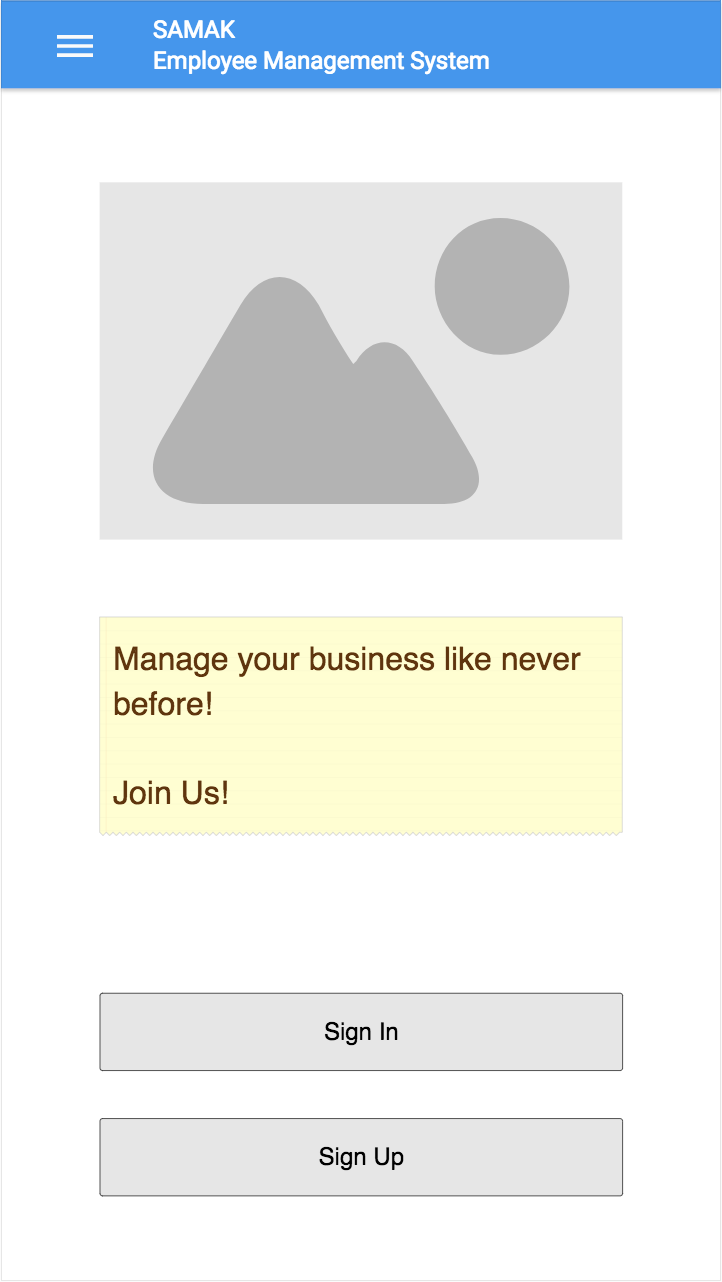
\includegraphics[width = 0.5\textwidth]{images/1-main-page.png}
\end{center}

این صفحه مثالی از صفحه‌ی اصلی نهایی سامانه را نشان می‌دهد.
از طریق این صفحه می‌توان به کاربرد‌های ورود به سامانه و تشکیل حساب کاربری دسترسی داشت.

\subsection{صفحه‌ی ورود به سامانه}


\begin{center}
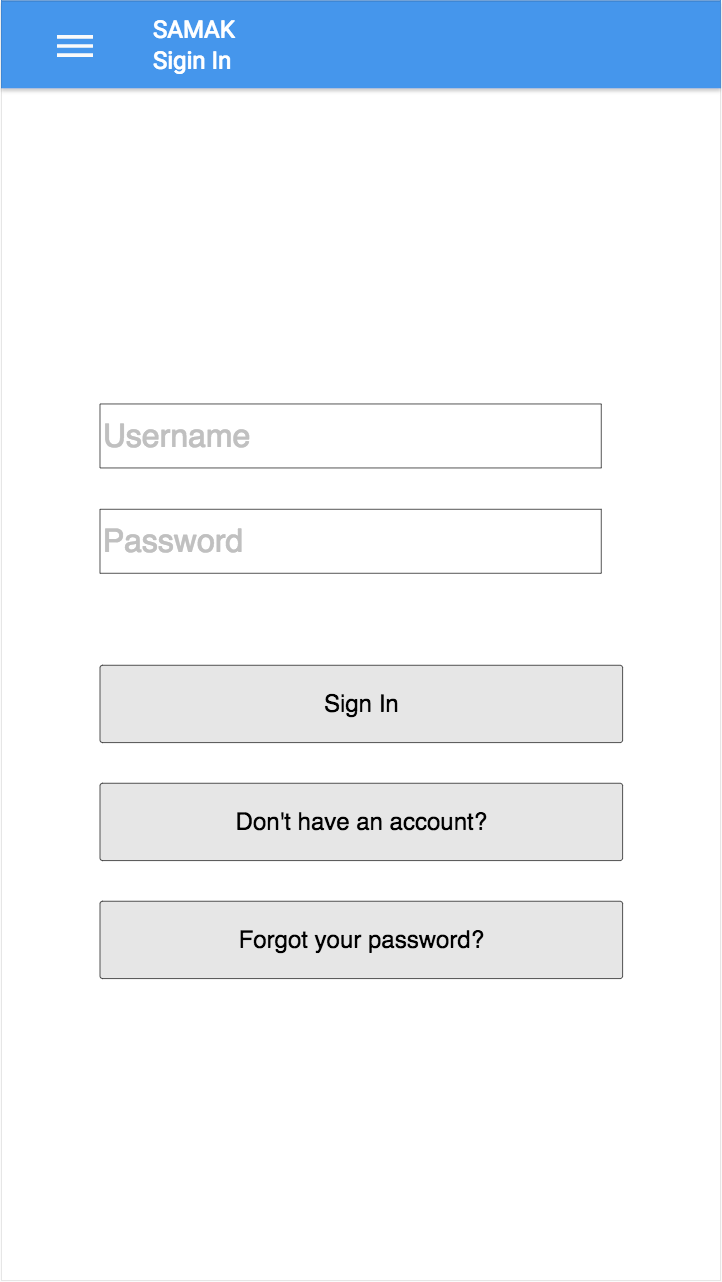
\includegraphics[width = 0.5\textwidth]{images/2-sign-in.png}
\end{center}


این صفحه، صفحه‌ی ورود به سامانه است، از طریق این صفه می‌توان با ارائه کردن نام کاربری و کلمه‌ی عبور وارد سامانه شد.
در صورتی که نیاز به تشکیل حساب کاربری باشد می‌توان از طریق این صفحه، به صفحه‌ی ساخت حساب کاربری ناوبری کرد.

در صورتی که کلمه‌ی عبور فراموش شده باشد نیز می‌توان با استفاده از این صفحه وارد صفحه‌ی فراموشی کلمه‌ی عبور شد.

با اتمام فرایند ورود به سامانه کاربر به صورت خودکار به صفحعه‌ی حساب کاربری منتقل خواهد شد.

\subsection{صفحه‌ی ثبت نام در سامانه}

\begin{center}
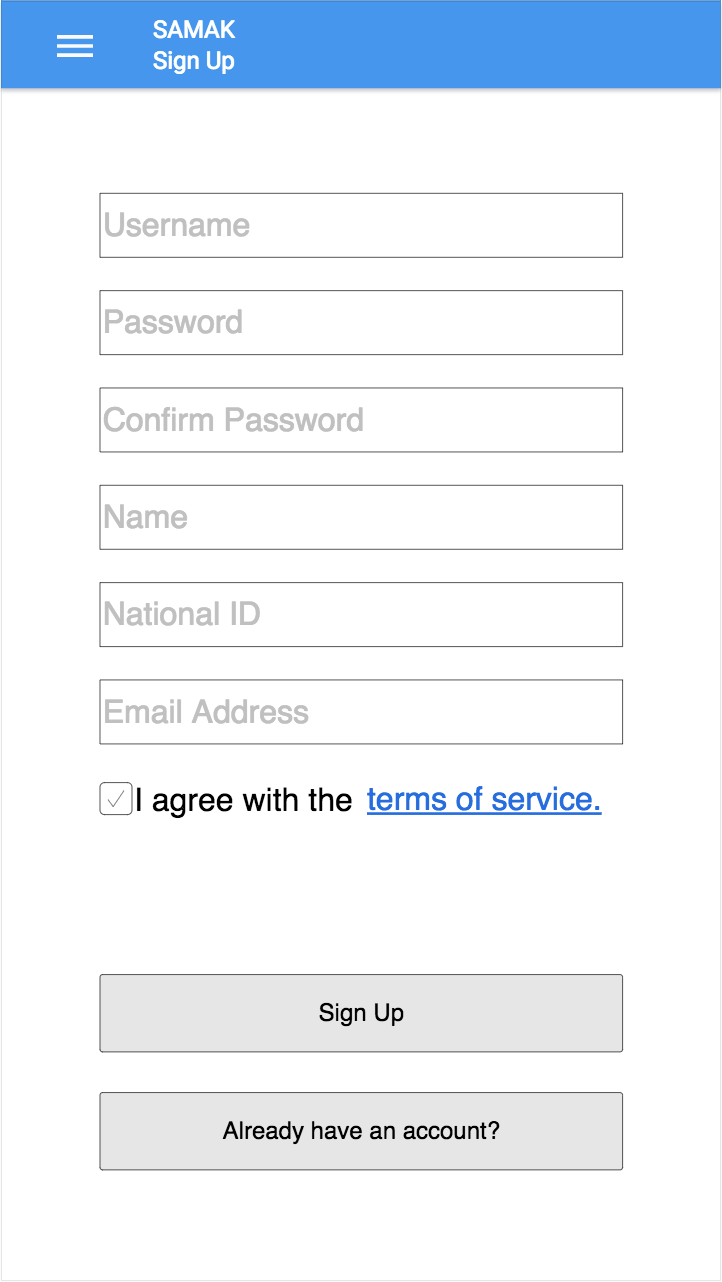
\includegraphics[width = 0.5\textwidth]{images/3-sign-up.png}
\end{center}

از طریق این صفحه می‌توان با وارد کردن مشخصات اقدام به ساخت حساب کاربری کرد. در صورتی که قبلا حساب کاربری ایجاد شده باشد می‌توان از طریق این صفحه به صفحه‌ی ورود به حساب کاربری ناوبری کرد.
با اتمام روند ثبت نام کاربر به صورت خودکار به صفحعه‌ی ورود به سامانه منتقل خواهد شد.


\subsection{صفحه‌ی فراموشی کلمه‌ی عبور - ۱}

\begin{center}
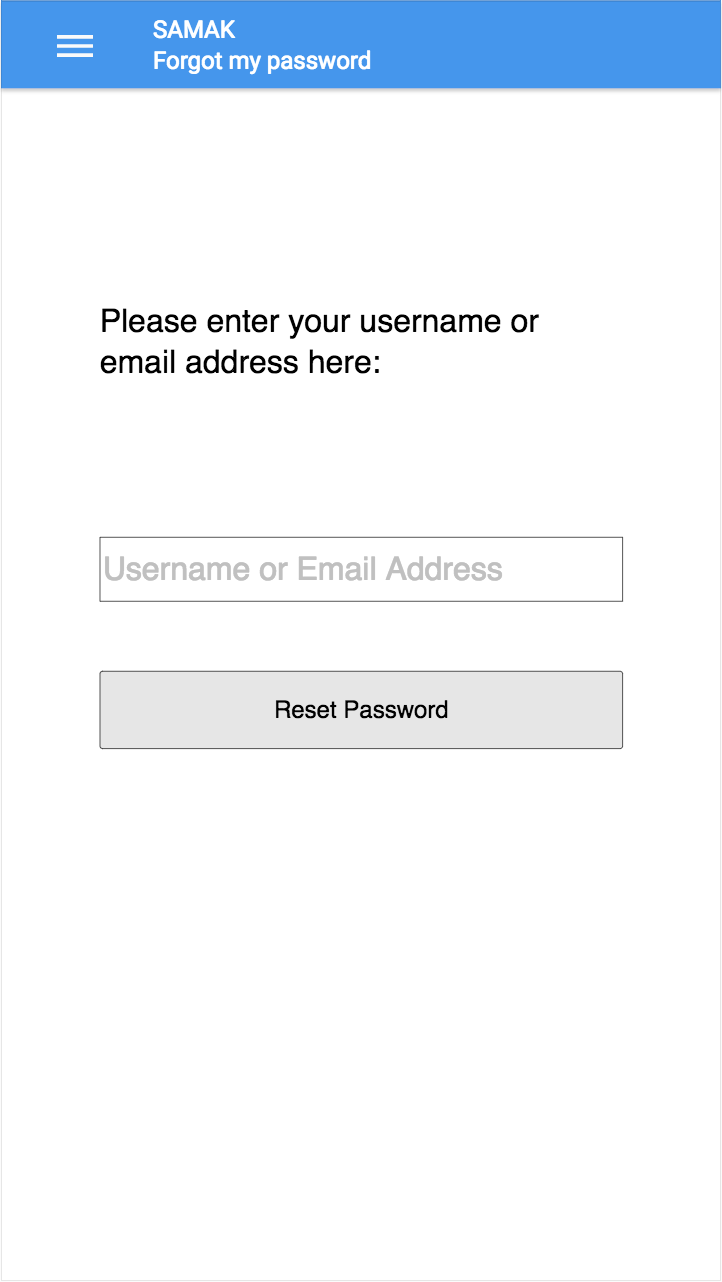
\includegraphics[width = 0.5\textwidth]{images/4-forgot-password-1.png}
\end{center}

در صورتی که کاربر کلمه‌ی عبور خود را فراموش کرده باشد می‌تواند از طریق این صفحه درخواست بازنشانی آن را صادر کند. به این صورت با وارد کردن نام کاربری یا ایمیل خود، ایمیلی از طریق سامانه حاوی کدی جهت بازنشانی کلمه‌ی عبور به وی فرستاده می‌شود.  پس از ثبت درخواست کاربر به صفحه‌ی ورود کد بازنشانی منتقل می‌شود. از این صفحه و در صورتی که کد بارنشانی درست وارد شود، به صفحه‌ی تعیین کلمعه‌ی عبور جدید منتقل می‌شود که در آن می‌تواند نسبت به تعیین کلمه‌ی عبور جدید اقدام کند.

در نهایت با پایان فرایند، کاربر به صفحه‌ی ورود منتقل خواهد شد.





\subsection{صفحه‌ی فراموشی کلمه‌ی عبور - ۲}
\begin{center}
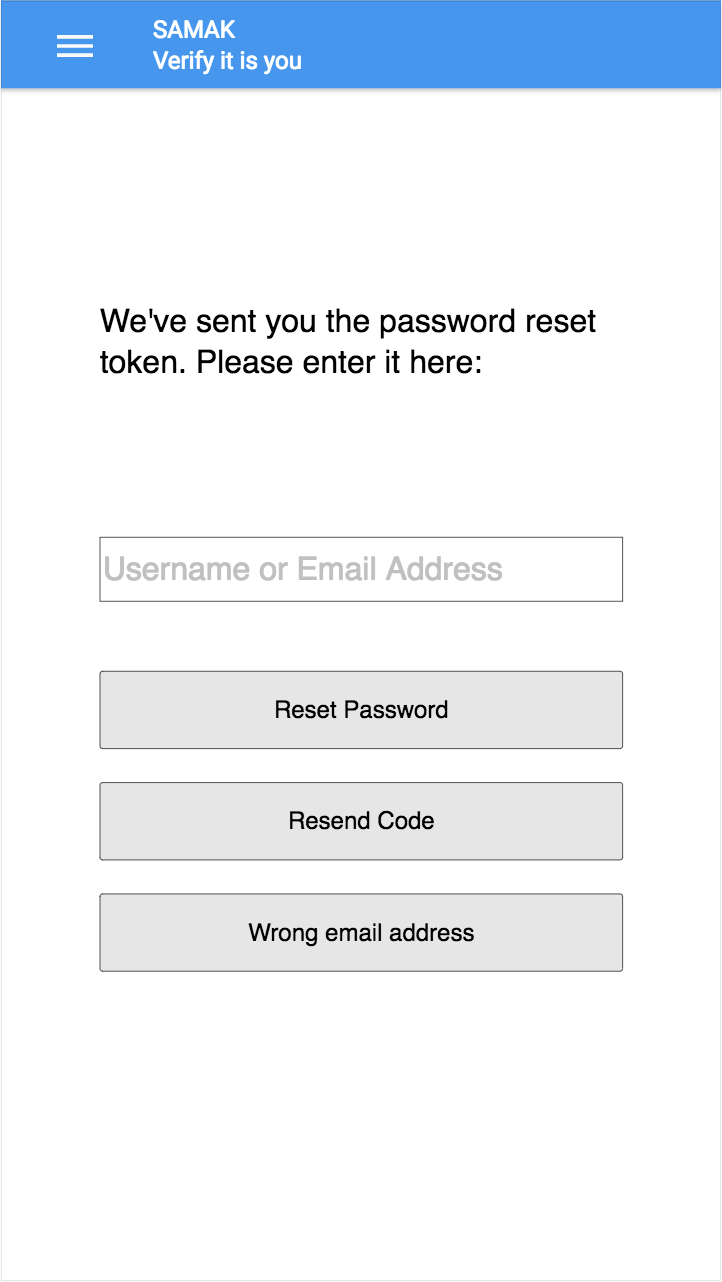
\includegraphics[width = 0.5\textwidth]{images/5-forgot-password-2.png}
\end{center}







\subsection{صفحه‌ی فراموشی کلمه‌ی عبور - ۳}

\begin{center}
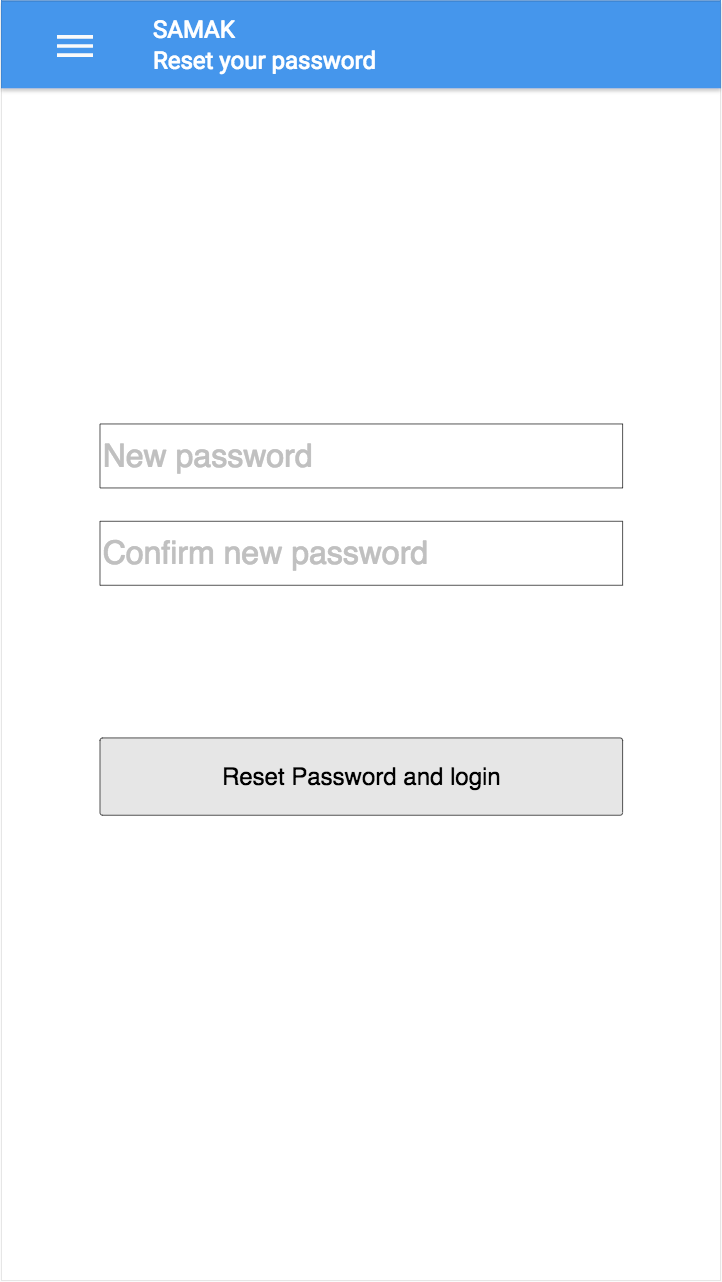
\includegraphics[width = 0.5\textwidth]{images/6-forgot-password-3.png}
\end{center}



\subsection{صفحه‌ی حساب کاربری}


\begin{center}
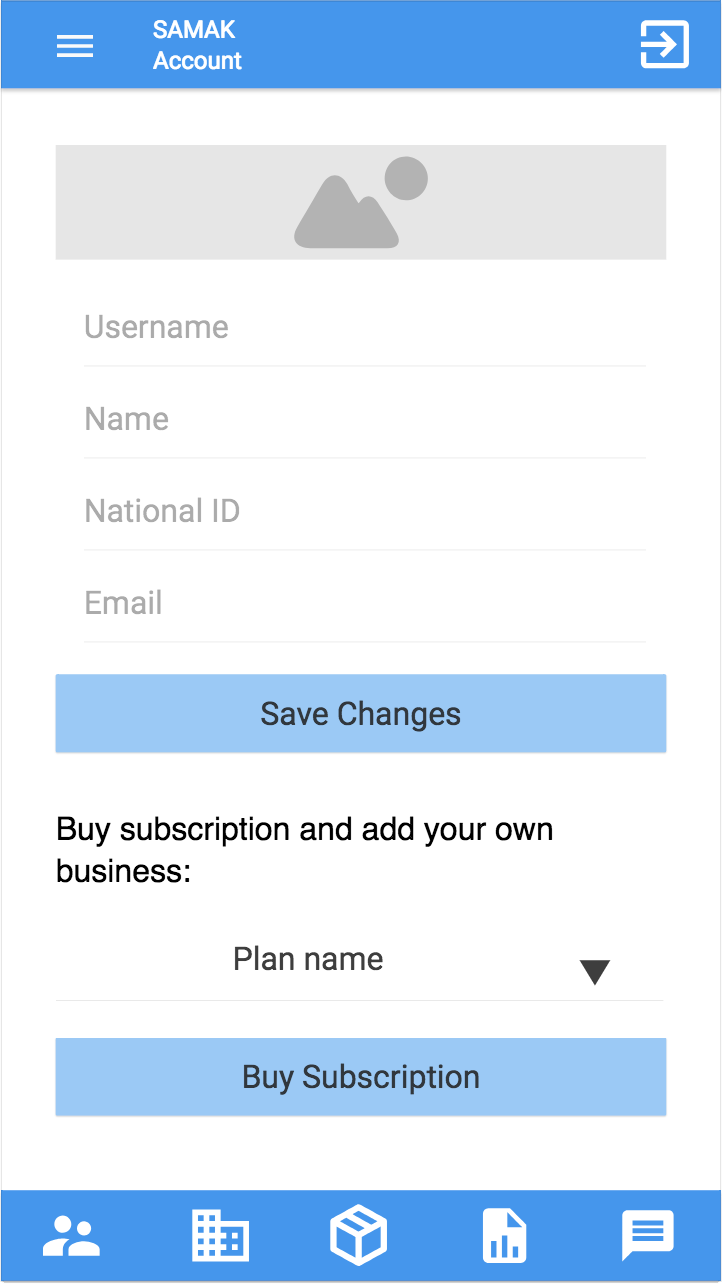
\includegraphics[width = 0.5\textwidth]{images/7-account.png}
\end{center}

کاربر از طریق این صفحه می‌توان نسبت به تغییر مشخصات حساب کاربری خود اقدام کند. در پایین صفحه برای کاربرانی که مدیر کسب و کار نباشند گزینه‌ی خرید اشتراک سامانه به نمایش در خواهد آمد که از طریق آن می‌توانند نسبت به ارتقای حساب کاربری خود به حساب مدیریتی اقدام کنند.


\subsection{صفحه‌ی کسب و کار}


\begin{center}
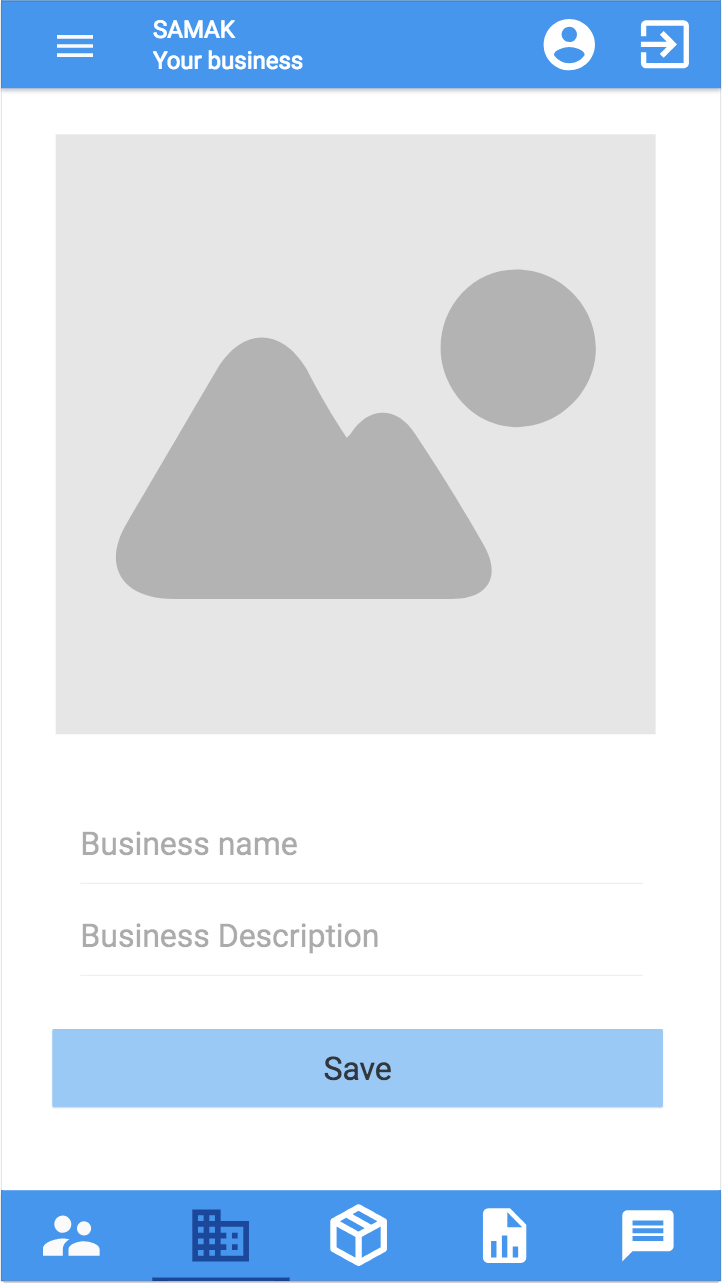
\includegraphics[width = 0.5\textwidth]{images/8-business.png}
\end{center}


کاربران از طریق این صفحعه می‌توانند اطلاعات کسب و کار جدید خود را تعیین کرده اطلاعات فعلی را ویرایش کنند.

با انتخاب گزینه‌ی ذخیره سازی کاربر به صفحه‌ی کارکنان منتقل خواهد شد.


\subsection{صفحه‌ی کارکنان}

\begin{center}
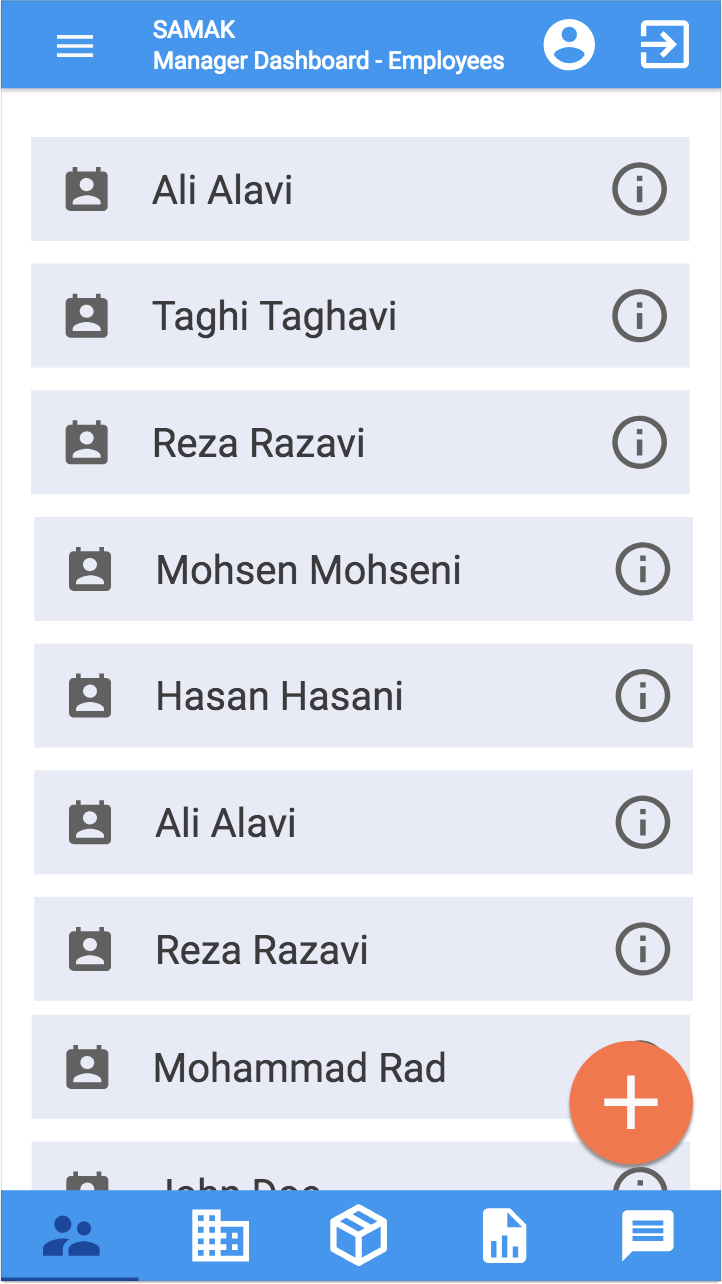
\includegraphics[width = 0.5\textwidth]{images/9-employees.png}
\end{center}

از طریق این صفحه کاربر می‌توان اطلاعات هر یک از کارکنان خود را دیده، آنها را ویرایش کند، کارمند جدید را به کسب و کار خود دعوت کند یا کارمندان فعلی را حذف کند.

دسترسی به امکان اضافه کردن کارمند جدید از طریق دکمه‌ی action در پایین صفحه میسر شده است. برای دریافت باقی امکانات، کاربر بایستی کارمند مورد نظرش را انتخاب کند.


\subsection{صفحه‌ی دعوت کارمند}

\begin{center}
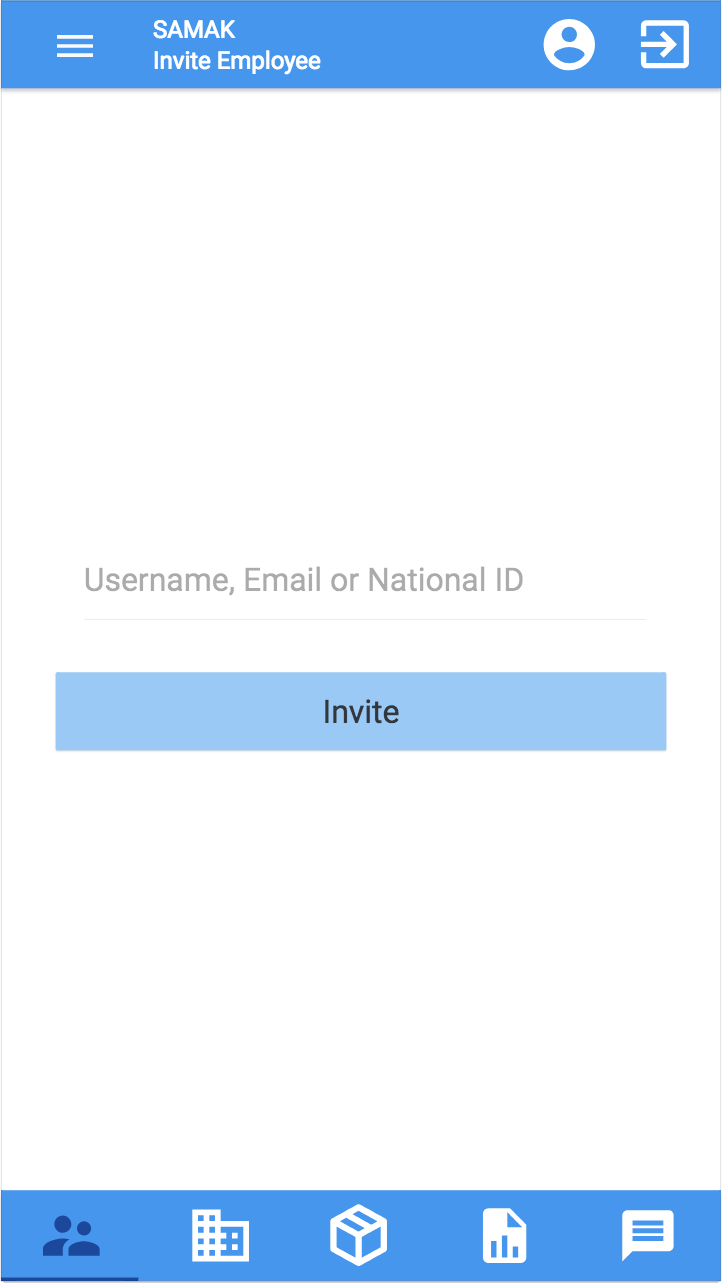
\includegraphics[width = 0.5\textwidth]{images/10-new-employee.png}
\end{center}

از این صفحه برای دعوت کارمند جدیدبه کسب و کار با ارائه‌ی کد ملی، نام کاربری یا آدرس ایمیل می‌توان استفاده کرد.

دعوت نامه در بخش request  ها در زیرسیتم پیام رسانی نمایش داده خواهد شد که فرد هدف می‌تواند آن را بپذیرد یا رد کند.


\subsection{صفحه‌ی مشخصات کارمند }

\begin{center}
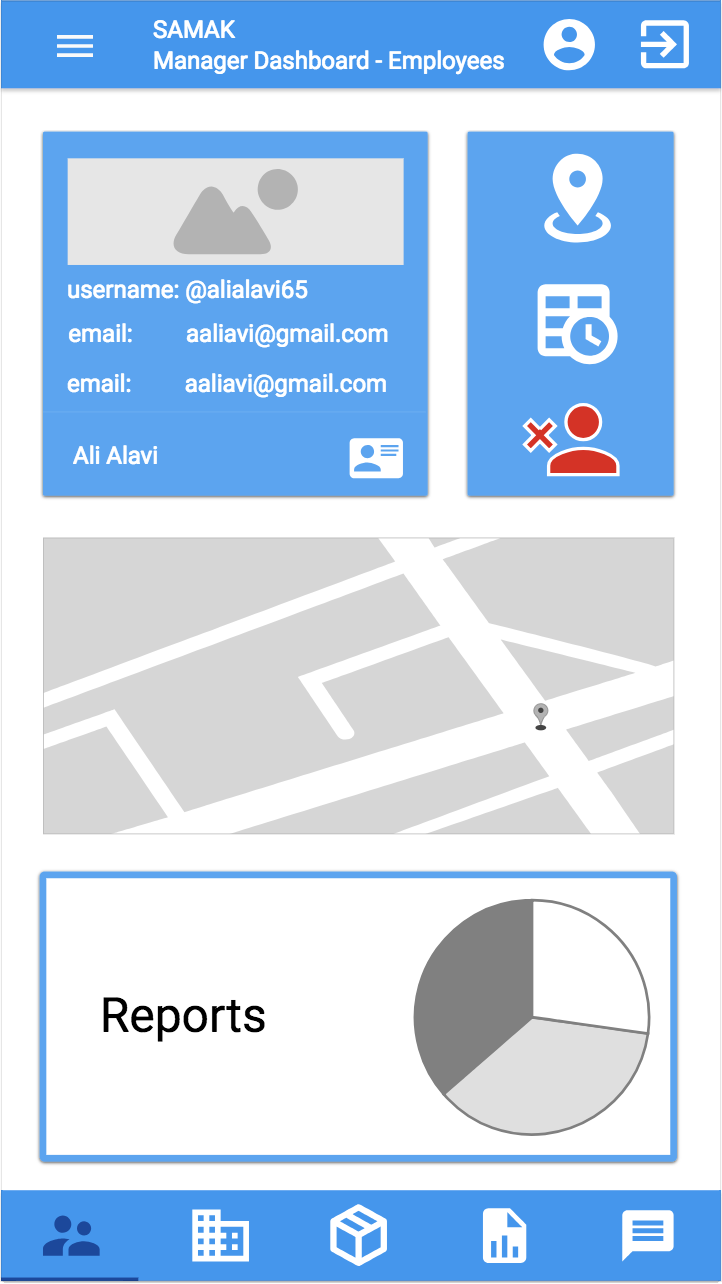
\includegraphics[width = 0.5\textwidth]{images/11-employee-details.png}
\end{center}

از طریق این صفحه می‌توان به صورت متمرکز به مشخصات کارمند دسترسی داشت، در صورت لزوم آنها را ویرایش کرد، کارمند را از کسب و کار حذف کرد، به موقعیت فعلی کارمند دسترسی داشت، نسبت به ثبت ردیاب برای کارمند اقدام کرد، برنامه‌ی شیفت کاری کارمند را تنظیم کرد و به گزارشات موردی و دقیق تر در مورد او دسترسی داشت.




\subsection{صفحه‌ی گزارشات کارمند}
\begin{center}
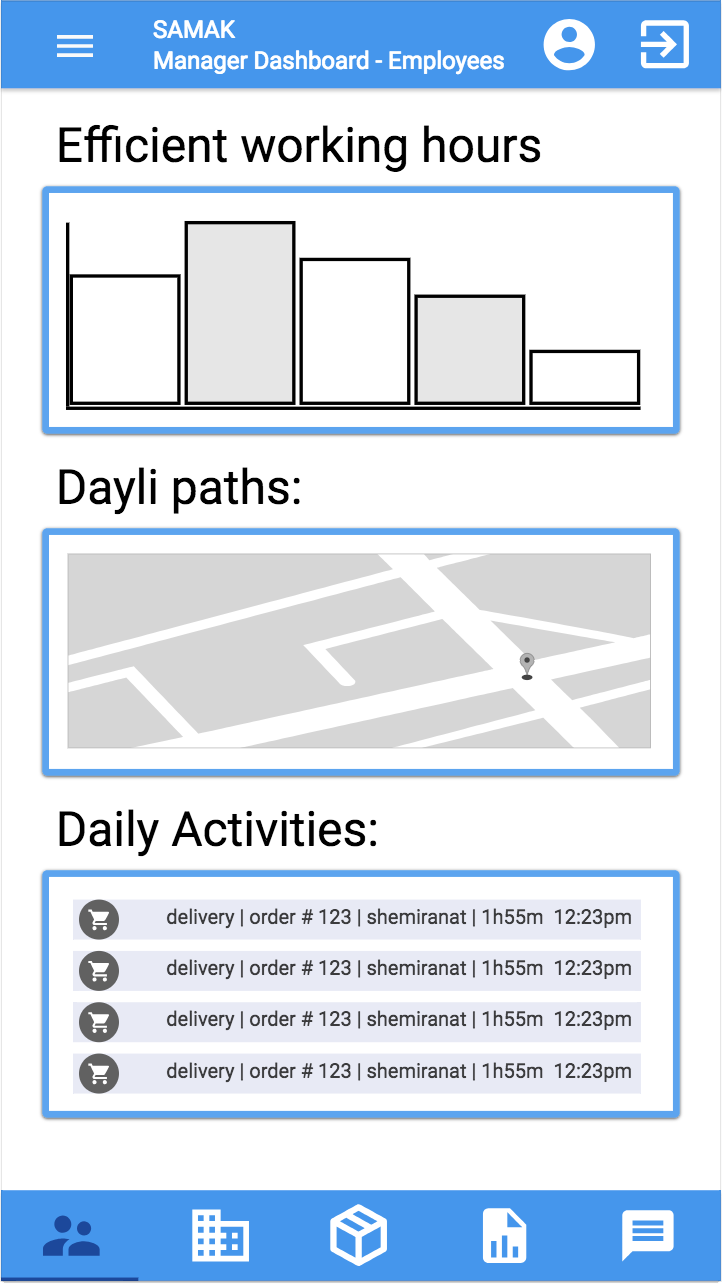
\includegraphics[width = 0.5\textwidth]{images/12-employee-reports.png}
\end{center}


از طریق این صفحه می‌توان به گزارشات کاری کارمند مانند ساعات کاری مفید، مسیر‌های پیموده شده و فعالیت‌های انجام شده دسترسی داشت.


\subsection{صفحه‌ی سفارشات}

\begin{center}
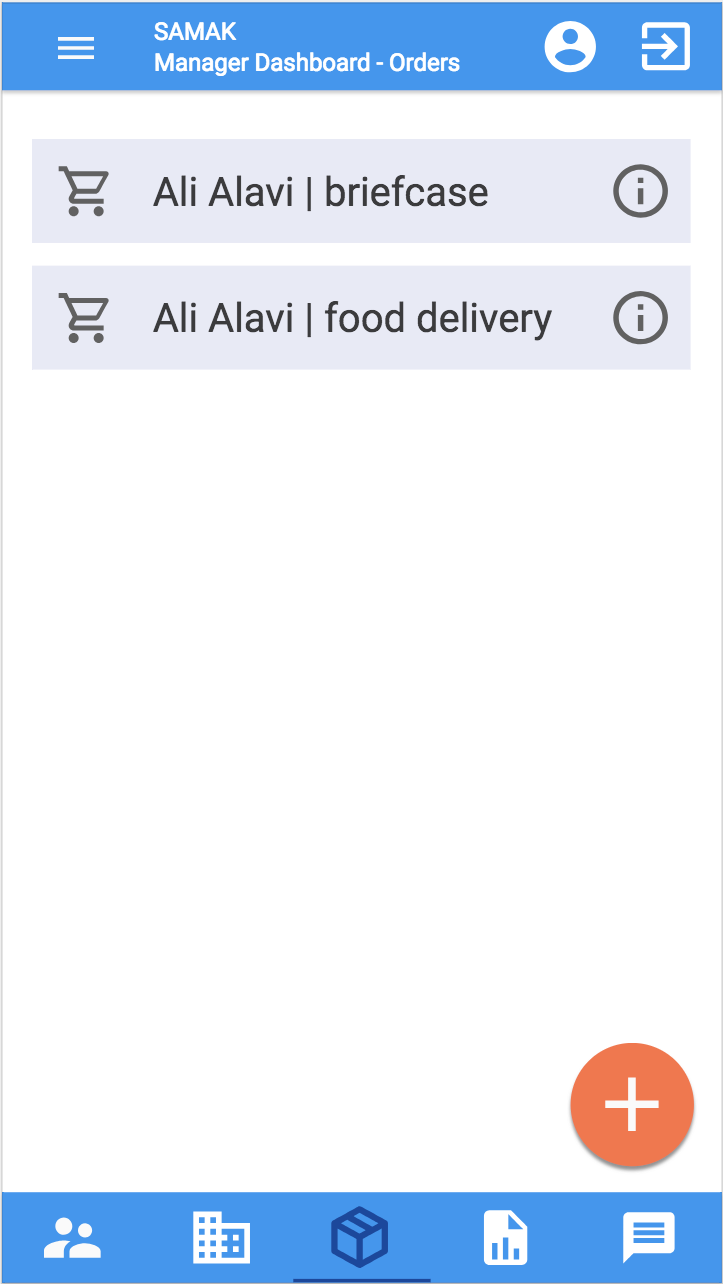
\includegraphics[width = 0.5\textwidth]{images/13-orders.png}
\end{center}

مدیر کسب و کار می‌تواند از طریق این صفحه نسبت به ثبت سفارش جدید و مشاهده و ویرایش سفارشات قبلی اقدام کند.



\subsection{صفحه‌ی ثبت سفارش جدید یا ویرایش سفارش فعلی}

\begin{center}
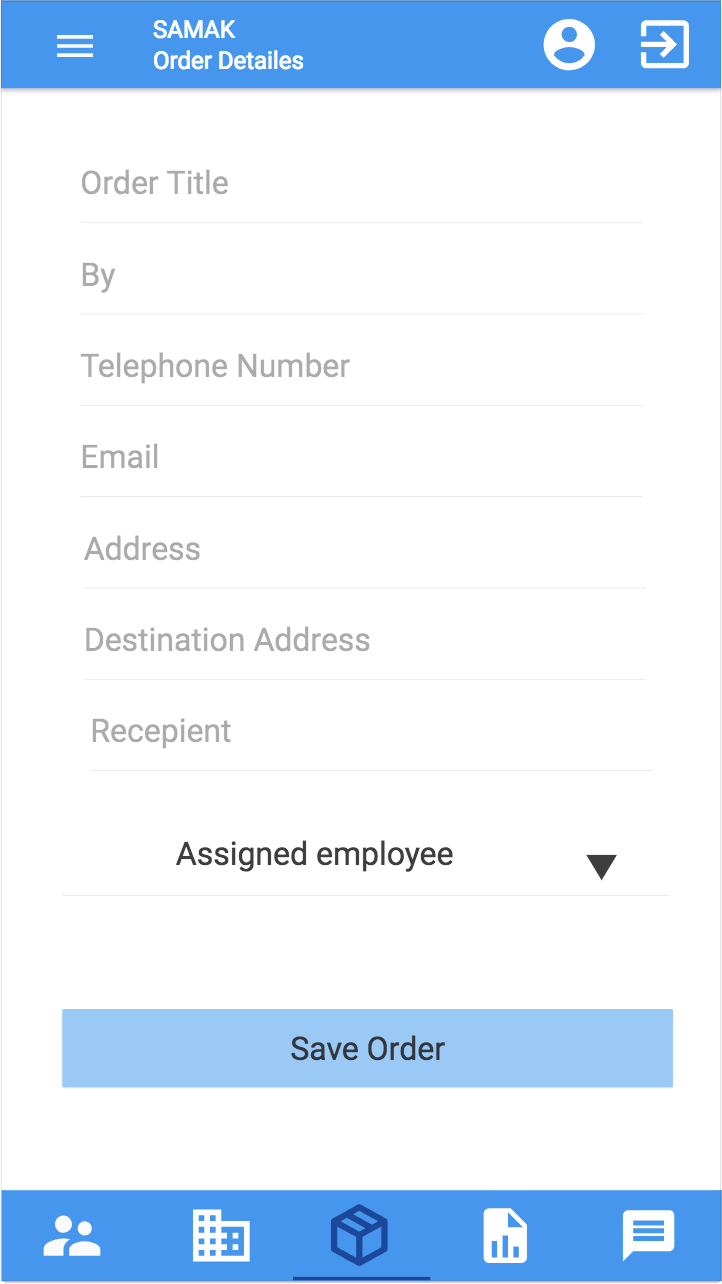
\includegraphics[width = 0.5\textwidth]{images/14-new-order-edit-order.png}
\end{center}

در صورتی که گزینه‌ی ثبت سفارش جدید انتخاب شود یا ویرایش یک سفارش فعلی انتخاب شود، به این صفحه ناوبری خواهیم کرد. در این صفحعه کاربر اطلاعات یا تغییرات مورد نظر خود را وارد کرده و در صورت لزوم سفارش را به یک کارمند الصاق می‌کند.


\subsection{صفحه‌ی جزئیات سفارش}

\begin{center}
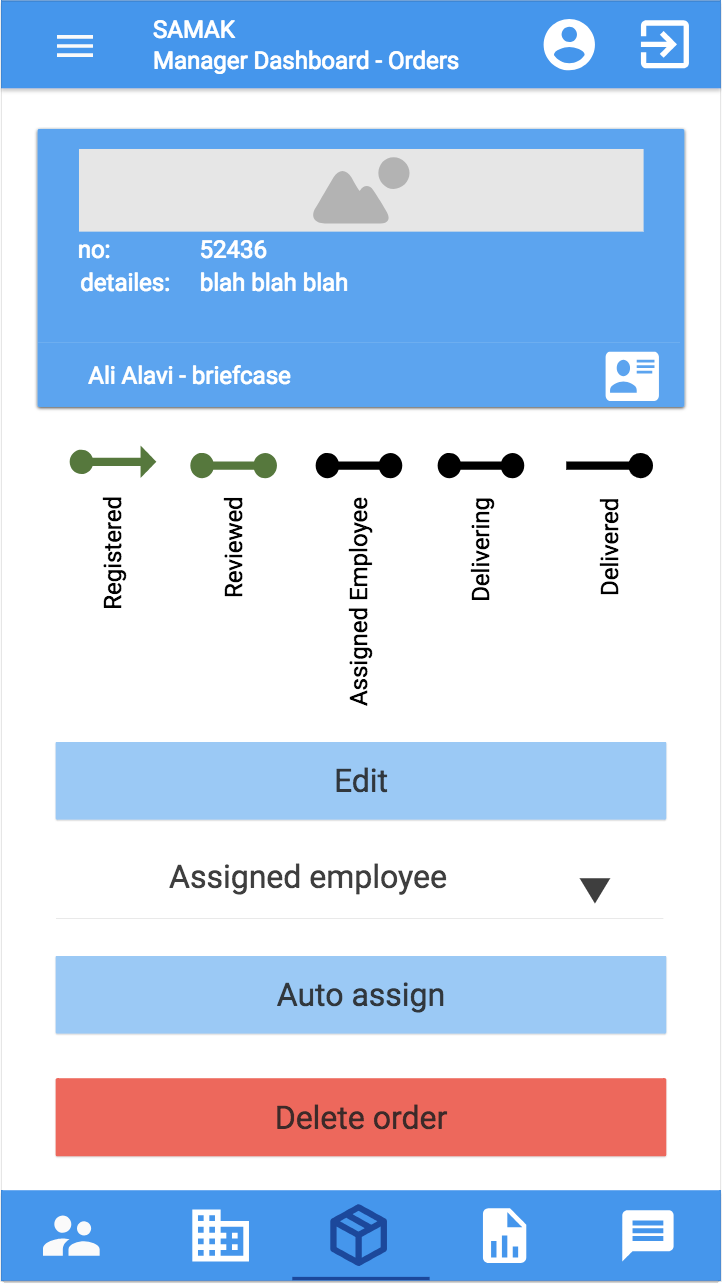
\includegraphics[width = 0.5\textwidth]{images/15-order-details.png}
\end{center}


از طریق این صفحه می‌توان به اطلاعات سفارش و اطلاعات مراحل انجام سفارش  دسترسی داشت و آنها را مشاهده و در صورت لزوم ویرایش کرد.

از طریق این صفحه می‌توان کارمندی را  برای انجام سفارش انتخاب کرد یا انتخاب خودکار بهترین کارمند را برگزید.

همچنین می‌توان در صورت لزوم سفارش را حذف کرد.


\subsection{صفحه‌ی گزارش گیری}

\begin{center}
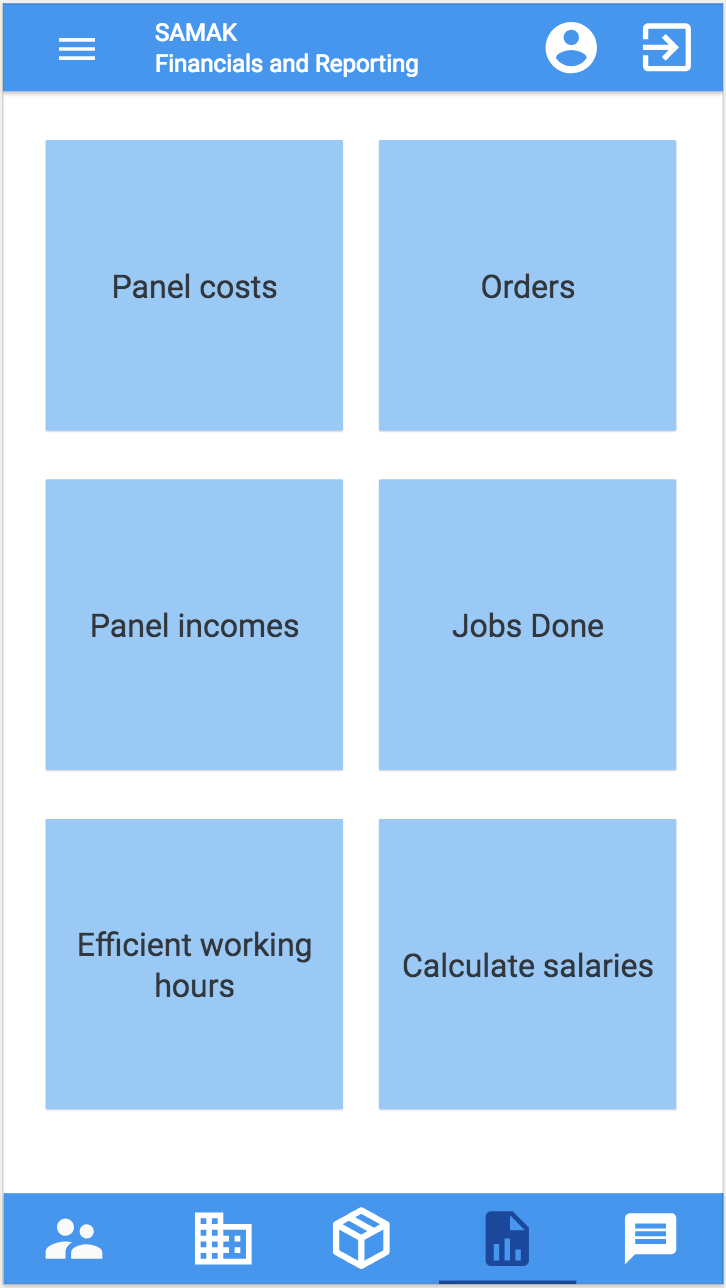
\includegraphics[width = 0.5\textwidth]{images/15-reports.png}
\end{center}

در این صفحه، مدیر کسب و کار می‌تواند به انواع گزارشات مالی و کسب و کاری دسترسی داشته باشد.



\subsection{صفحه‌ی پیام رسانی مدیر}

\begin{center}
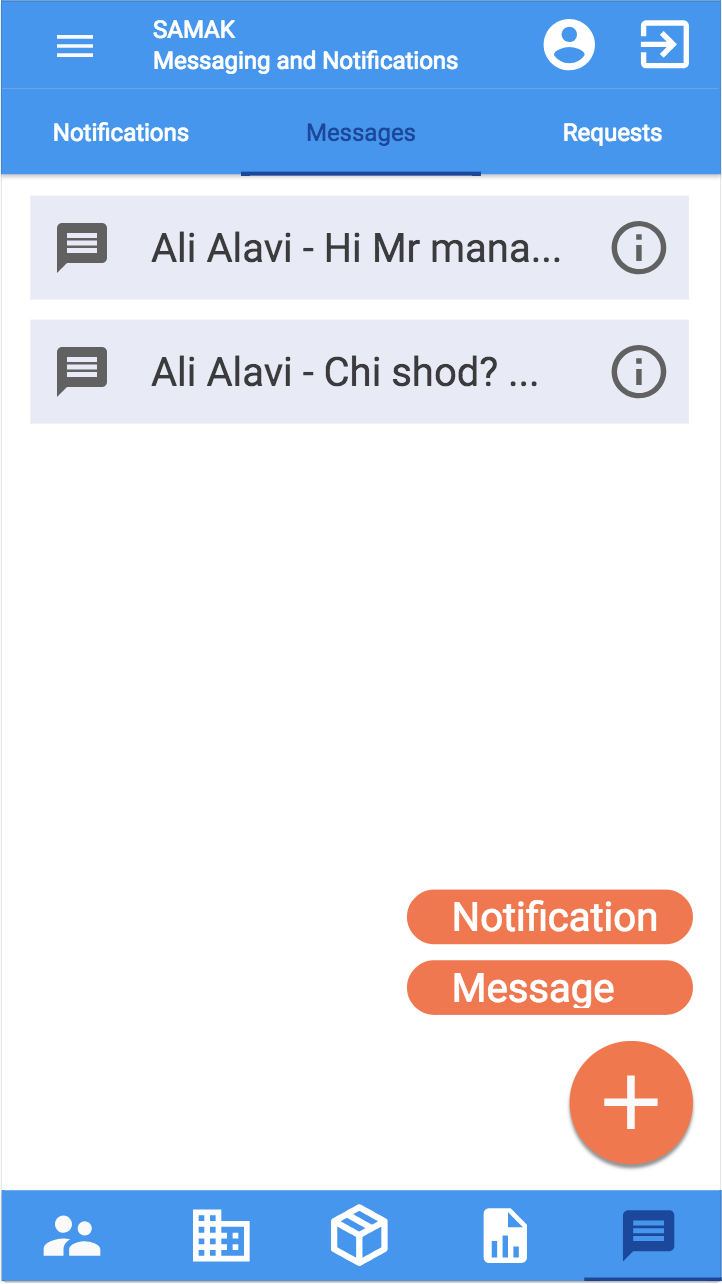
\includegraphics[width = 0.5\textwidth]{images/16-messaging-manager.png}
\end{center}

از طریق این صفحه مدیر می‌تواند به ایجاد خصوصی یا اعلان عمومی جدید مبادرت کند. همچنین مدییر می‌تواند از بخش درخواست‌ها، درخواست‌های کارکنان خود را دیده و در صورت لزوم تایید یا رد کند.



\subsection{صفحه‌ی پیام رسانی کارمند}


\begin{center}
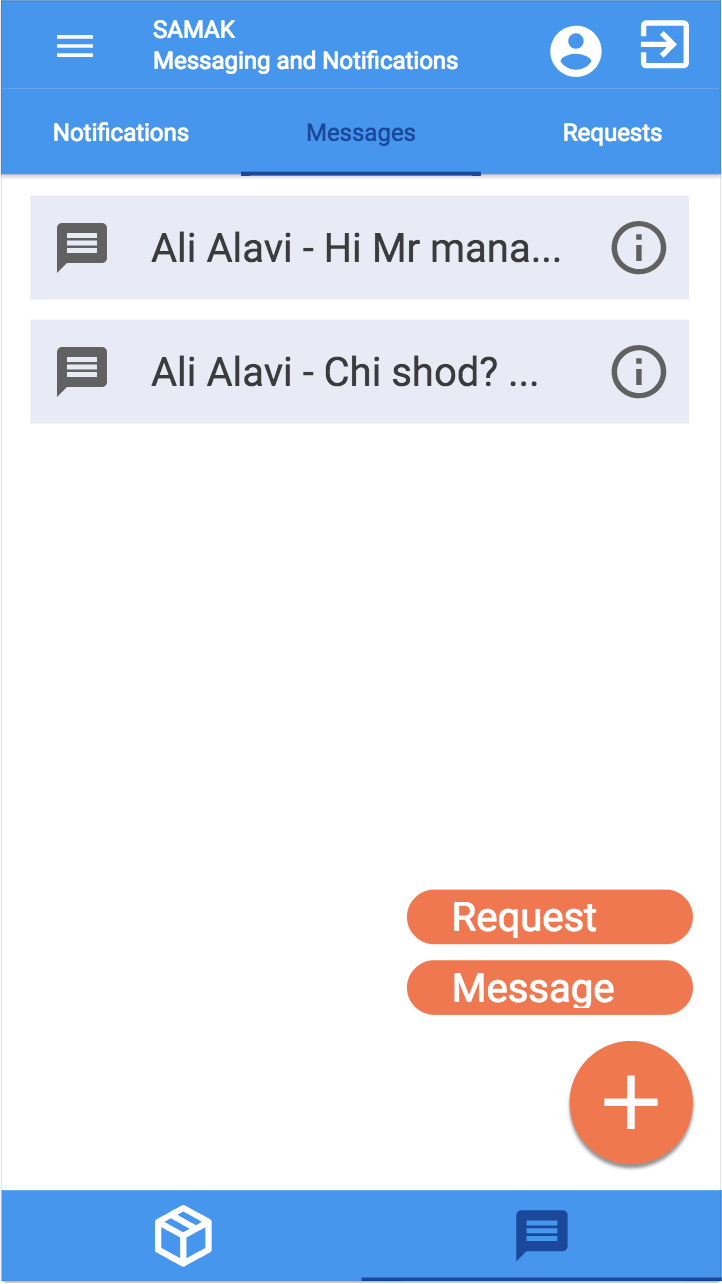
\includegraphics[width = 0.5\textwidth]{images/17-messaging-employee.png}
\end{center}

از طریق این صفحه کارمند می‌تواند به ایجاد خصوصی یا درخواست جدید مبادرت کند. همچنین دعوت‌نامه‌های عضویت در کسب و کار در بخش درخواست‌ها به کاربر نمایش داده می‌شوند که می‌تواند آنها را تایید یا رد کند.

\subsection{صفحه‌ی مشاهده‌ی پیام}

\begin{center}
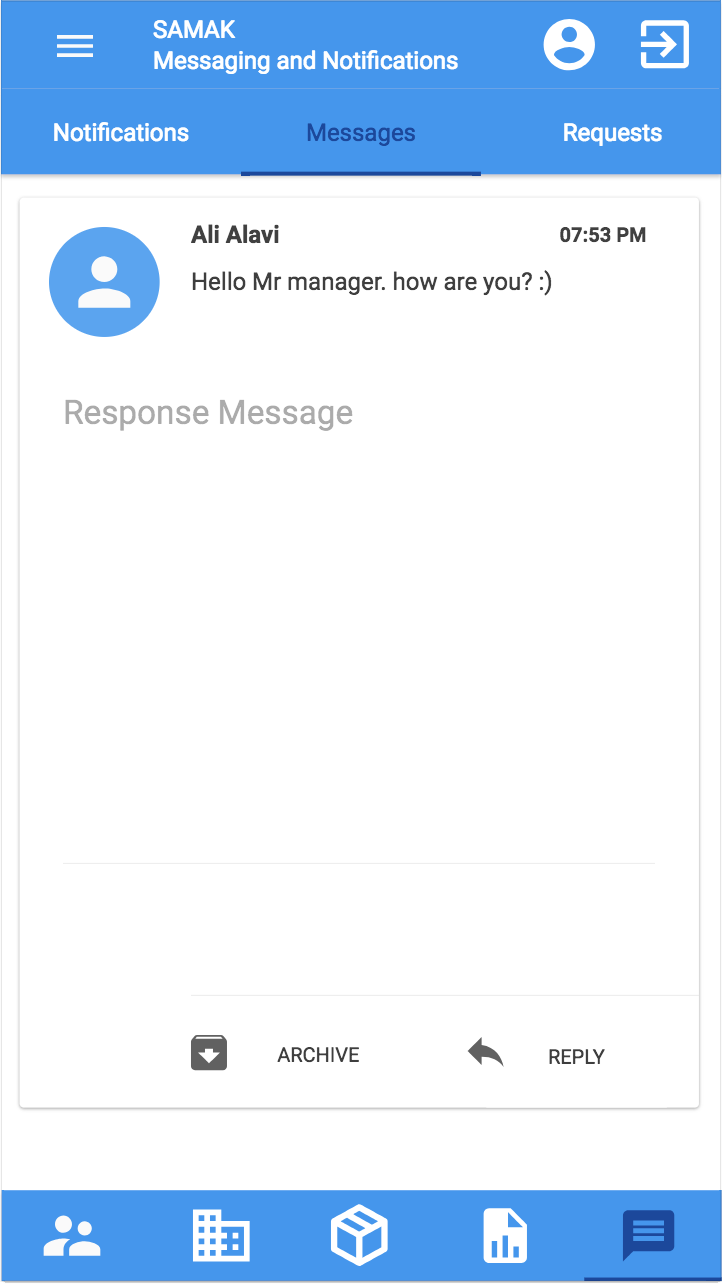
\includegraphics[width = 0.5\textwidth]{images/18-view-message.png}
\end{center}

کاربران سامانه می‌توانند از طریق این صفحه، پیام‌های دریافتی را مشاهده کرده، در صورت نیاز پاسخ دهند و یا حذف کنند.


\subsection{صفحه‌ی مشاهده‌ی اعلان}

\begin{center}
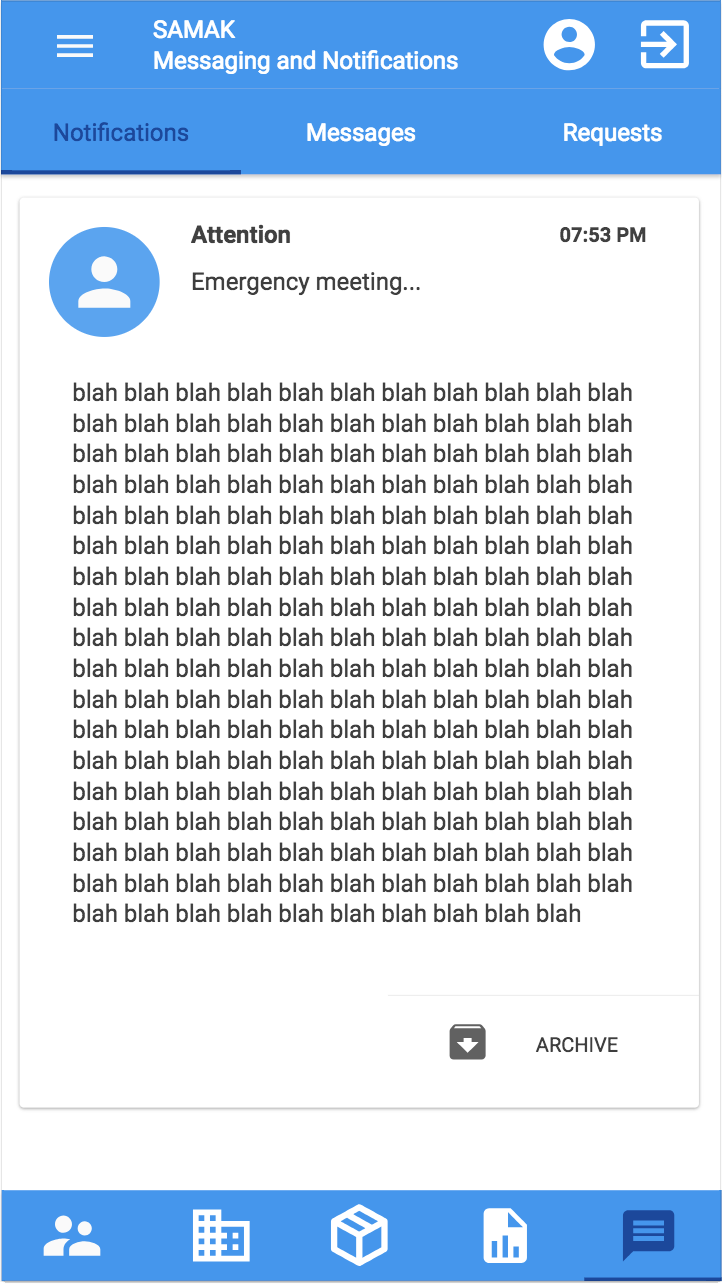
\includegraphics[width = 0.5\textwidth]{images/19-view-announcement.png}
\end{center}

کاربران سامانه می‌توانند از طریق این صفحه، اعلان‌های دریافتی را مشاهده کرده،  و در صورت تمایل حذف کنند.



\subsection{صفحه‌ی ایجاد پیام}

\begin{center}
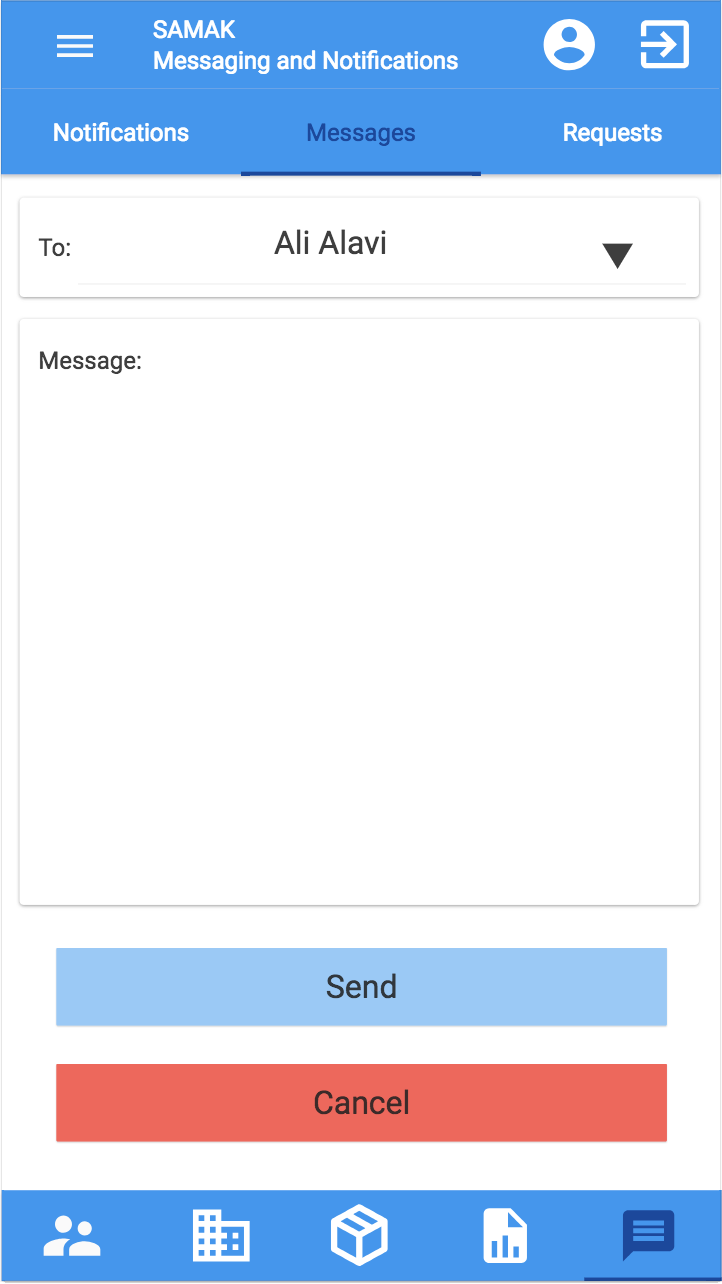
\includegraphics[width = 0.5\textwidth]{images/20-reply-delete.png}
\end{center}

کاربران سامانه می‌توانند از طریق این صفحه نسبت به ایجاد پیام جدید اقدام کنند. به این منظور بایستی گیرنده‌ی پیام و متن آن را وارد کنند.


\subsection{صفحه‌ی ایجاد درخواست}

\begin{center}
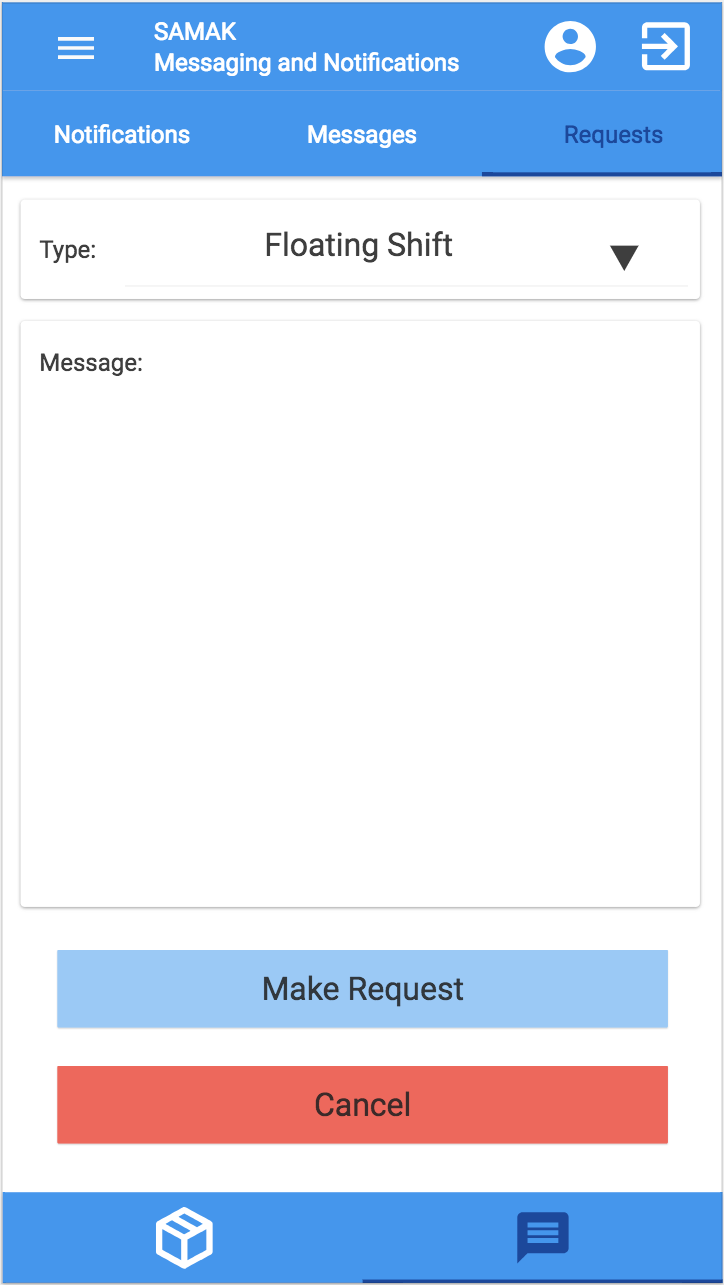
\includegraphics[width = 0.5\textwidth]{images/21-make-request.png}
\end{center}

کارمندان می‌توانند از طریق این صفحه نسبت به طرح درخواست‌هایی پیش فرض یا شخصی به مدیریت اقدام کنند.


\subsection{صفحه‌ی پاسخ درخواست}

\begin{center}
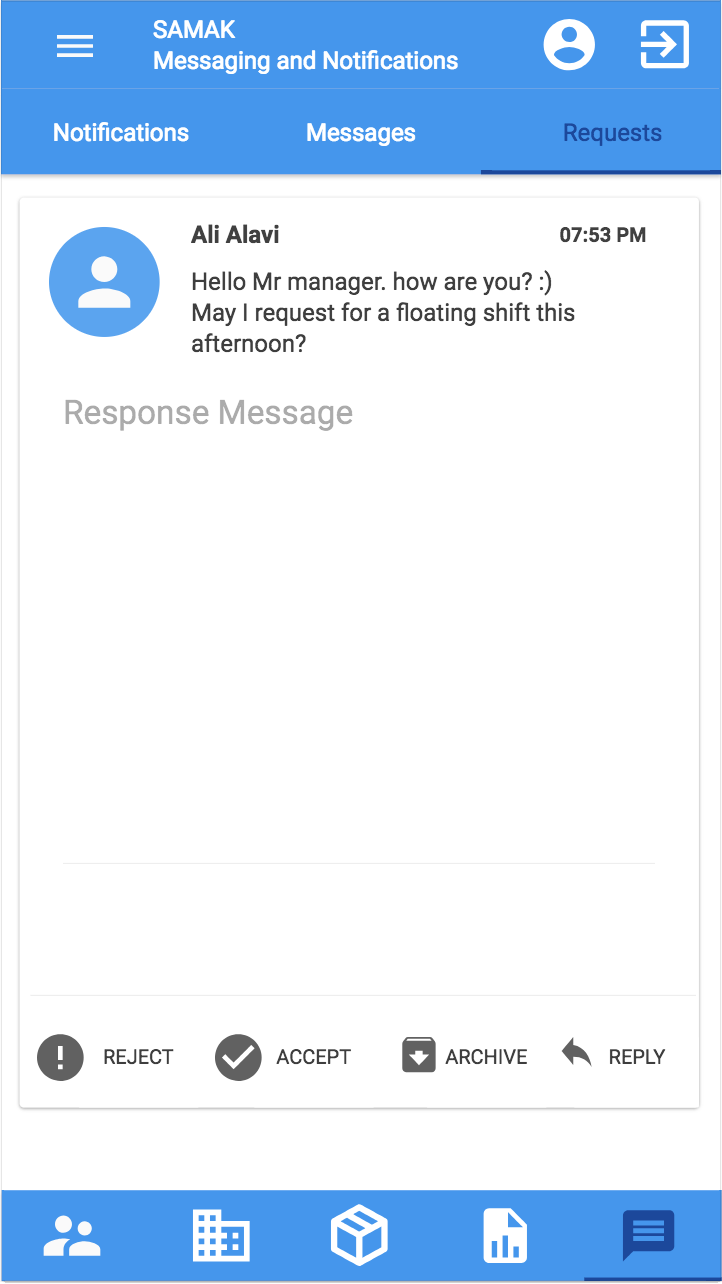
\includegraphics[width = 0.5\textwidth]{images/22-answer-request.png}
\end{center}

مدیریت کسب و کار می‌تواند از طریق این بخش‌، درخواست‌های دریافتی از کارمندان را پاسخ گفته، حذف کرده، تایید و یا رد کند.



